\chapter{Charge Readout Planes}
\label{ch:fddp-CRP}

%%%%%%%%%%%%%%%%%%%%%%%%%%%%%%%%%%%%%%%%%%%%%%%%%%%%%%%%%%%%%%%%%%%%
\section{Charge Readout Planes (CRP) Overview}
\label{sec:fddp-crp-ov}


%%%%%%%%%%%%%%%%%%%%%%%%%%%%%%%%%
\subsection{Introduction}
\label{sec:fddp-crp-intro}

In the dual-phase LArTPC concept, the ionization electrons are multiplied in avalanches  occurring inside micro-pattern detectors, the Large Electron Multipliers (LEMs), located in the argon gas  phase above the liquid argon level. The drift field of the TPC brings the electrons up to the liquid argon surface where they can  be    extracted into the gas using a 2-kV/cm electric field defined across the liquid-gas interface.

This extraction field is defined by the potentials applied to submersed extraction grid (stainless steel wires tensioned in both $x$ and $y$ directions) and to the bottom side of the LEMs. The LEMs are printed circuit boards oriented horizontally, with conductive layers (electrodes) on the top and bottom surfaces, and many holes drilled through.  The holes form a micro-pattern structure within which the amplification occurs given the presence of a strong electric field.

By applying voltages across the two electrodes of the LEM, an electric field region (up to 35 kV/cm) is defined in the holes, allowing to achieve a gain exceeding 20 after the initial phase of  charging-up the LEM dielectric material. The nominal operation conditions correspond to a again of 20 after charging-up. Electrons transiting these high electric field regions in the holes trigger Townsend multiplication in the pure argon gas.

The amplified charge is then collected and recorded on a 2D anode consisting of two sets of 3.125-mm-pitch gold-plated copper strips that provide the $x$ and $y$ coordinates (and thus two orthogonal views) of the event. The strips are defined by a pattern of tracks on the bottom face of the anode printed circuit board. It is possible  to define two electrically insulated views of strips crossing each other orthogonally be ensuring continuity of the tracks with a set of vias and tracks extending to the top face of the anode printed circuit board.

Typical electric fields between each stage of the readout are
illustrated in Figure~\ref{fig:setup}. Table~\ref{tab:crp_dist} shows the inter-stage distance and the tolerances required to obtain uniformity of gain to within $\sim$5\%.

\begin{dunefigure}[Dual-phase readout]{fig:setup}
{Illustration of the electric fields in the amplification region of a dual-phase LArTPC. The simulated field lines in dark blue indicate the paths followed by the drifting charges (without diffusion).}
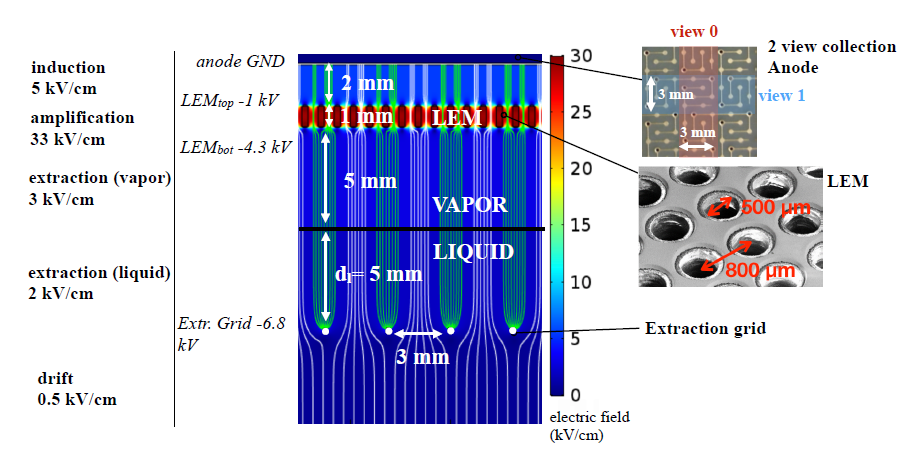
\includegraphics[width=.85\textwidth]{amplification-principle2.png}  
\end{dunefigure}
\begin{dunetable}[Interstage distances and electric field settings of the dual-phase readout components]{lp{2cm}p{2cm}l}{tab:crp_dist}{Interstage distances and electric field settings of the dual-phase readout components.} 
 Component & Distance [mm] & Tolerance [mm] & Electric field [kV/cm]  \\ \toprowrule
 Anode-LEM top electrode  & 2 & 0.1 & 5\\ \colhline
 LEM top-bottom electrode   & 1 & 0.01 & 30-35\\ \colhline
 LEM bottom electrode-grid        & 10 & 1 & 2 (in LAr) and 3 (in GAr)\\
 \end{dunetable}

The extraction grid, LEM and anode are assembled into three-layered ``sandwiches'' with precisely defined inter-stage distances and inter-alignment,  which are then connected together horizontally into modular units of area \num{9}~m$^2$. These units are called Charge Readout Planes (CRP). Figure~\ref{fig:figure-label-crp} shows an 
engineering view of one CRP fully assembled.

\begin{dunefigure}[optional caption for LoF]{fig:figure-label-crp}
{View of a complete CRP module of 9 m$^{2}$}
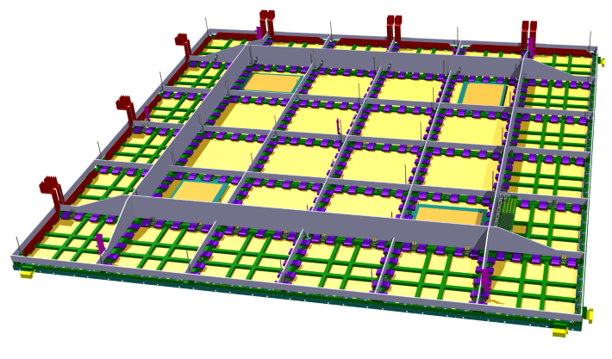
\includegraphics[width=0.75\textwidth]{CRP-fig1.png}
\end{dunefigure}

The CRP mechanical structure provides the integration of the LEM-anode sandwiches over a large area by minimizing the dead spaces. The planarity of the active surface must be guaranteed despite possible sagging effects with respect to the three hanging points, differential thermal contraction effects on the various  components and the presence of a temperature gradient in the gas phase which cold induce different thermal contractions as a function of the distance from the liquid surface. In order to solve these aspects the design is based on a supporting frame in INVAR. INVAR allows building a stiff supporting structure, extending vertically in the gas phase, with little sagging and little contraction effects. The LEM and anodes which are affected by a significant thermal contraction are integrated in a G10 planar structure which has similar contraction effects. The G10 structure is mechanically decoupled on the horizontal plane with respect to the INVAR structure  and it is free to slide during thermal contraction. 


%%%%%%%%%%%%%%%%%%%%%%%%%%%%%%%%%%%%%
\subsection{Design Considerations}
\label{sec:fddp-crp-des-consid}

Each CRP is an independent detector element that performs charge
extraction, multiplication and collection, and has its own high voltage system and independent signal feedthroughs. The entire area of the LEM and anode in a CRP is active. The position and the parallelism with respect to the liquid argon surface can be individually adjusted for each CRP.

The LEM and corresponding anode are mounted in units of 50$\times$50~cm$^2$, called LEM/Anode Sandwich (LAS) modules, before being assembled with an extraction grid into a CRP. Each anode in a LAS is segmented in 50-cm long $x$ and $y$ strips . Adjacent LAS anodes are bridged together to form readout strips of the required length by connecting short flat cables to KEL connectors soldered onto the top sides of the anodes. The signals from the last anode in each  strip chain are brought to feedthroughs mounted on the other side of the front-end electronics embedded inside dedicated signal-feedthrough chimneys using 50-cm-long flat cables.

Each CRP is independently hung from the vessel deck through its three
suspension feedthroughs. It has its own high voltage system and  independent signal and slow-control feedthroughs.

The Charge Readout Planes design has been driven by a set of parameters and requirements which are summarised in Table~\ref{tab:crpphysicsparams} 

\begin{dunetable}
[Important parameters for the CRP system design]
{p{0.8\textwidth}}
{tab:crpphysicsparams}
{Important parameters for the CRP system design}   
Parameter \\ \toprowrule
 Planarity tolerance on the detection plane over 3x3m$^{2}$  $\pm$0,5mm \\ \colhline
 CRP vertical positioning precision  $\pm$0,5mm \\ \colhline
 Range of vertical displacement is $\pm$20mm\\ \colhline
 Lateral inter CRP dead space  less than 10mm \\\colhline
 Distance between the extraction grid wires and the LEM plane: 10mm\\ \colhline 
 High voltage of the extraction grid wires in liquid Argon: 6.8 kV \\ \colhline
 High voltage of the LEM down surface in gas argon: 4.5 kV\\ \colhline
 High voltage of the LEM up surface in gas argon: 1 kV\\ \colhline
\end{dunetable}

The CRP design foreseen for the DP detector module is based on the one developed for Proto-DUNE DP.

%%%%%%%%%%%%%%%%%%%%%%%%%%%%%%%%
\subsection{Scope}
\label{sec:fddp-crp-scope}

The scope of the Charge Readout Planes includes the continued procurement of materials for, and the fabrication, testing, delivery and installation of the following systems: 

\begin{itemize}
\item  Production and QA of the LEM and anodes
\item  Production of the G10 and INVAR frames
\item Production of the suspension feedthroughs and motorization
\item Production of the extraction grid elements
\item Production of the HV distribution system associated to the CRP to apply voltages to the LEM and anodes
\item Production of the system of temperature probes associated to the CRP
\item Production of the system of level meters associated to the CRP
\item Production of the system to pulse the strips associated to the CRP
\item Production of the transportation and storage boxes for the CRPs
\item Assembly of the LEM-anode sandwiches
\item Assembly of the CRP structures, LEM anode-sandwiches, grid elements, HV, slows control and cabling for each CRP
\item Testing of the assembled CRP
\item Installation in the storage boxes of the produced CRPs
\item Installation in the transportation boxes and delivery of the CRPs to be installed
\item Installation, cabling and test of the CRPs in the cryostat
\end{itemize}



%%%%%%%%%%%%%%%%%%%%%%%%%%%%%%%%%%%%%%%%%%%%%%%%%%%%%%%%%%%%%%%%%%%%
\section{CRP Design}
\label{sec:fddp-crp-design}

The complete CRP system includes, as illustrated in Figure~\ref{fig:figure-label-crp2}:
\begin{itemize}
\item Mechanical frames  
\item The detection plane made of LEM and Anodes 
\item The extraction grid
\item Instrumentation devices: level meters, distance meters, temperature probes
\item Internal cabling: to patch panels (LEM HV, slow control instruments)
\item Suspension and control system
\end{itemize}

\begin{dunefigure}[optional caption for LoF]{fig:figure-label-crp2}
{Main components of a CRP module of 9 m$^{2}$}
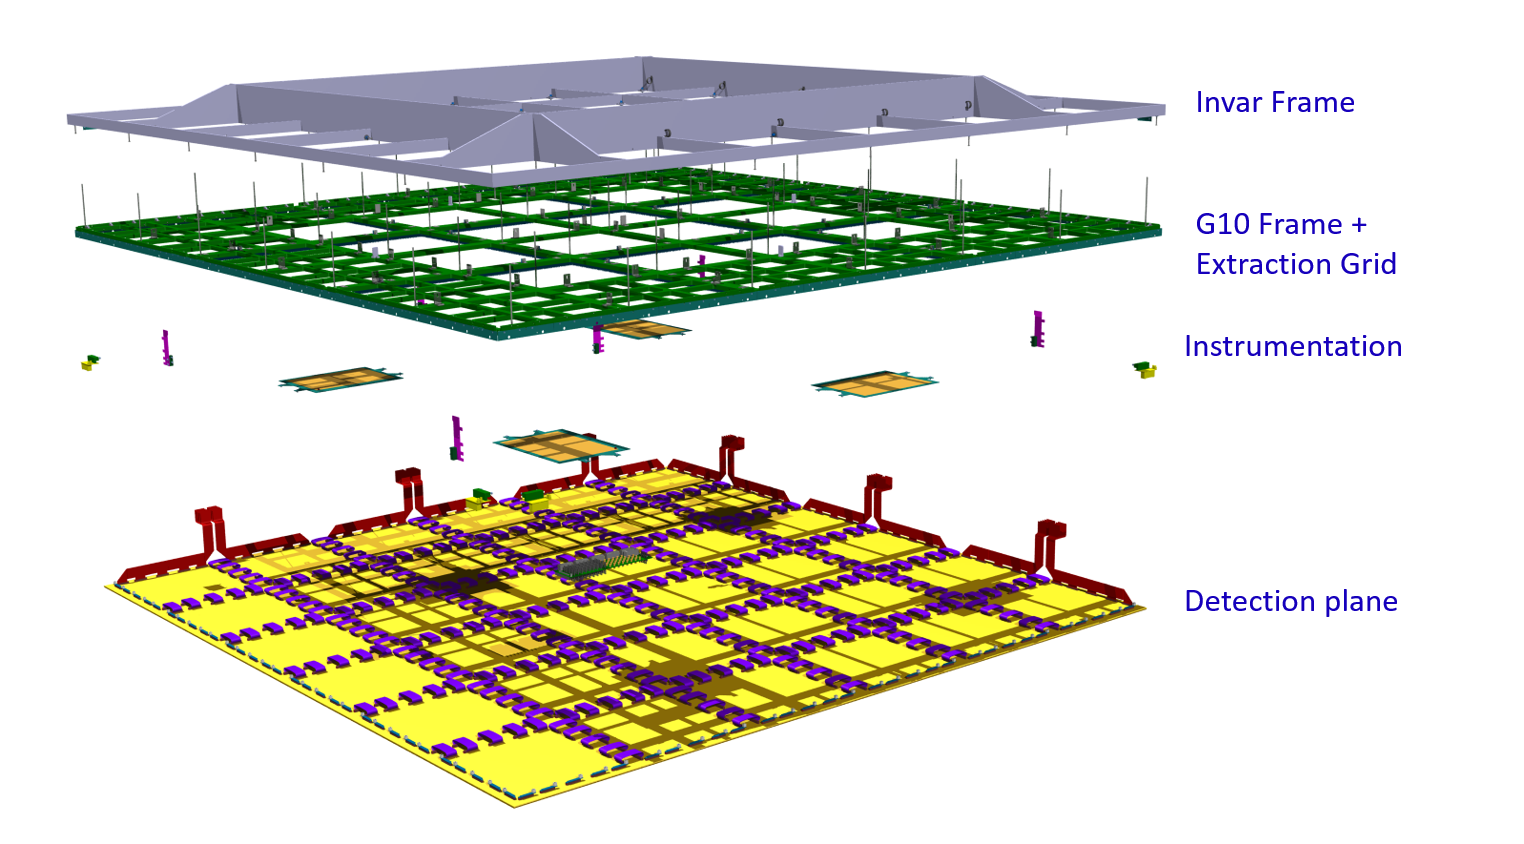
\includegraphics[width=0.8\textwidth]{CRP-fig2.png}
\end{dunefigure}

%%%%%%%%%%%%%%%%%%%%%%%%%%%%%%%%%%%
\subsection{Mechanical structure}
\label{sec:fddp-crp-mechanics}
\subsubsection{Invar frame}

The main mechanical supporting structure of the CRP is made of Invar Nickel-iron alloy. This material is chosen for its low coefficient of thermal expansion leading to a very small deformation at cold especially in the gas argon where the temperature gradient in the cryostat may be of the order of a few K/cm.
The structure is made of a grid of soldered Invar beams 3000 mm long and 6.5 mm wide. The four main ones have a height of 150 mm while the internal ones are 40 mm height as well as the 4 surrounding plates. The heights have been optimized to keep the stiffness as needed and to reduce the total frame weight which amounts to about 112 kg.
Figure~\ref{fig:invarframe} shows the soldering of one of the first CRP frame for ProtoDUNE-DP.
\begin{dunefigure}[optional caption for LoF]{fig:invarframe}
{First CRP invar frame under construction for ProtoDUNE-DP}
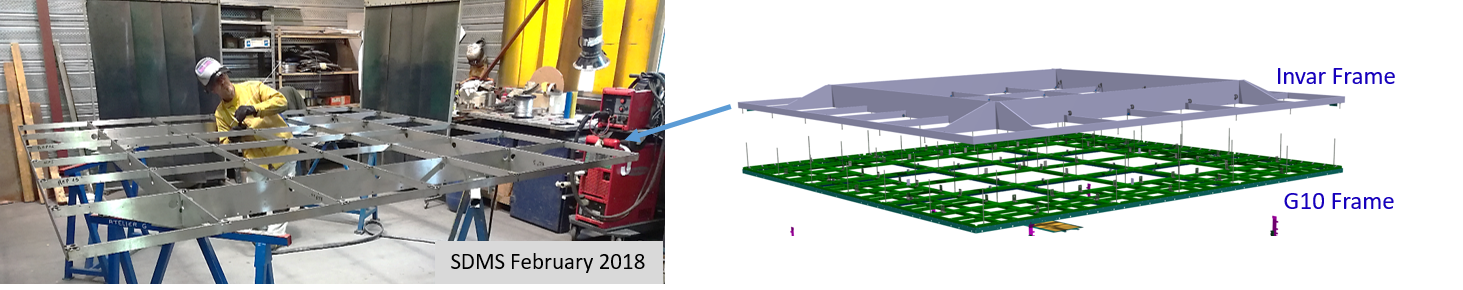
\includegraphics[width=0.95\textwidth]{invar-framev2.png}
\end{dunefigure}

\subsubsection{G10 frames and modules}

The 3x3 m G10 fiberglass structure used to attach the 36 LEM and Anodes, the extraction grid and the level meters is composed of an assembly of nine 1x1m$^2$ subframes. The choice of G10 is driven by the need to match the LEM and Anode thermo-mechanical behavior and avoid over-stress due to differential thermal contraction. 
Figure~\ref{fig:crp-g10} shows the pattern of the nine G10 parts composing a full CRP frame as well as the supporting comb positioned at every meter and the extraction grid support plates along the side of the CRP.

\begin{dunefigure}[optional caption for LoF]{fig:crp-g10}
{G10 elements of a full CRP module}
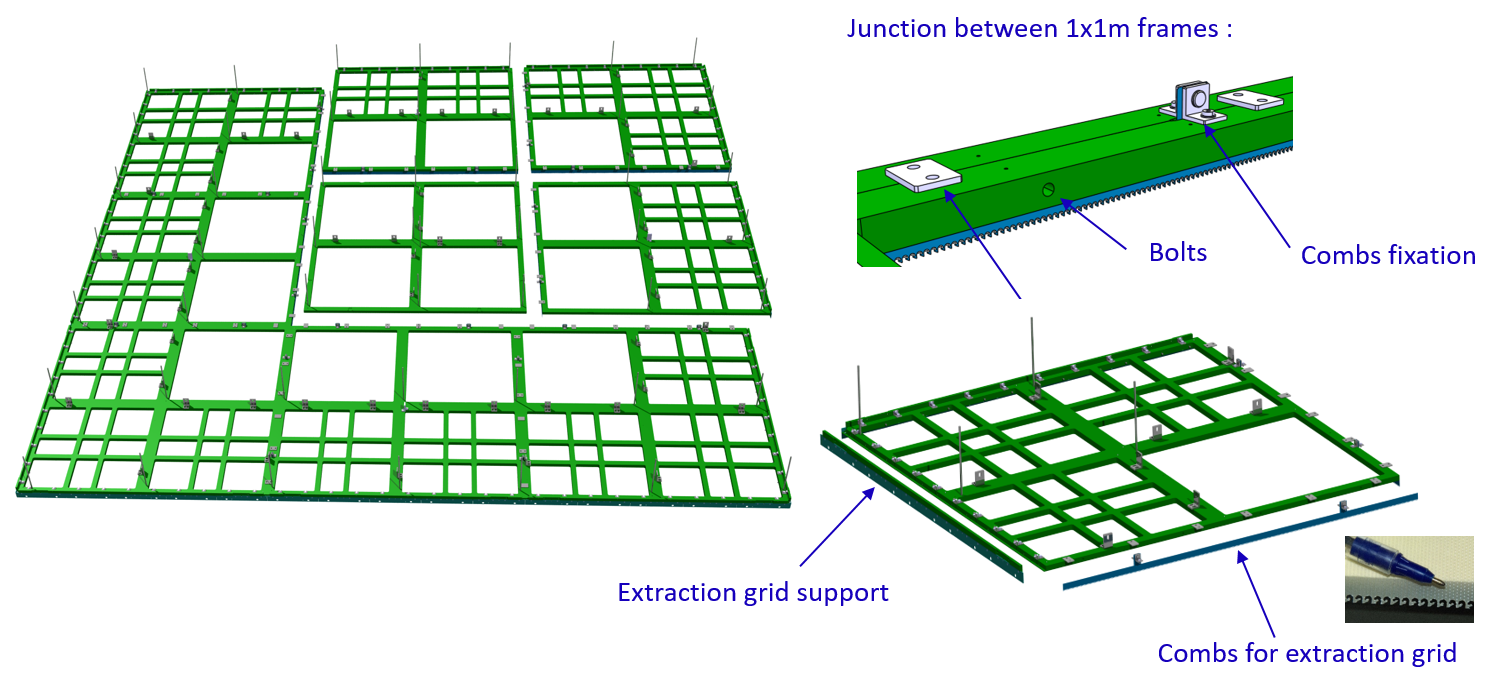
\includegraphics[width=0.8\textwidth]{G10.png}
\end{dunefigure}

Since G10 is a composite material created by stacking multiple layers of glass fibers,  the orientation of the stacking has to be taken into account prior to assembly.
At the construction level, the fiber directions are matched between the different subframes to insure harmony in thermal shrinkage. Three different patterns have to be produced, one for the four angles, one for the four face centers and one for the central subframe.
Two versions of each pattern for the supporting extraction grid bars and the combs follow same rule.

The design of the subframes have been calculated to guarantee enough stiffness in the  regions subject to larger tension with a minimum of material to reduce the weight.
The G10 structure is 15mm thick and weights about 68 kg. 

Differential thermal contraction occurs between G10 and Invar frames

\subsubsection{Decoupling system}
During cooling, Invar is nearly keeping its dimensions while G10 frame and LEMs/Anodes are contracting in similar ways. Thermal decoupling allows a lateral sliding of the G10 frame, without changing the altitude.
Dedicated decoupling systems are installed at each corner of the invar frame (50 systems by 3x3m module). One decoupling system allowing the sliding of G10+ LEM-anodes elements is shown in  Figure ~\ref{fig:crp-decoupling}.

\begin{dunefigure}[optional caption for LoF]{fig:crp-decoupling}
{Decoupling system attached to the invar frame with its detailed view. Example of one of the system built for ProtoDUNE-DP.}
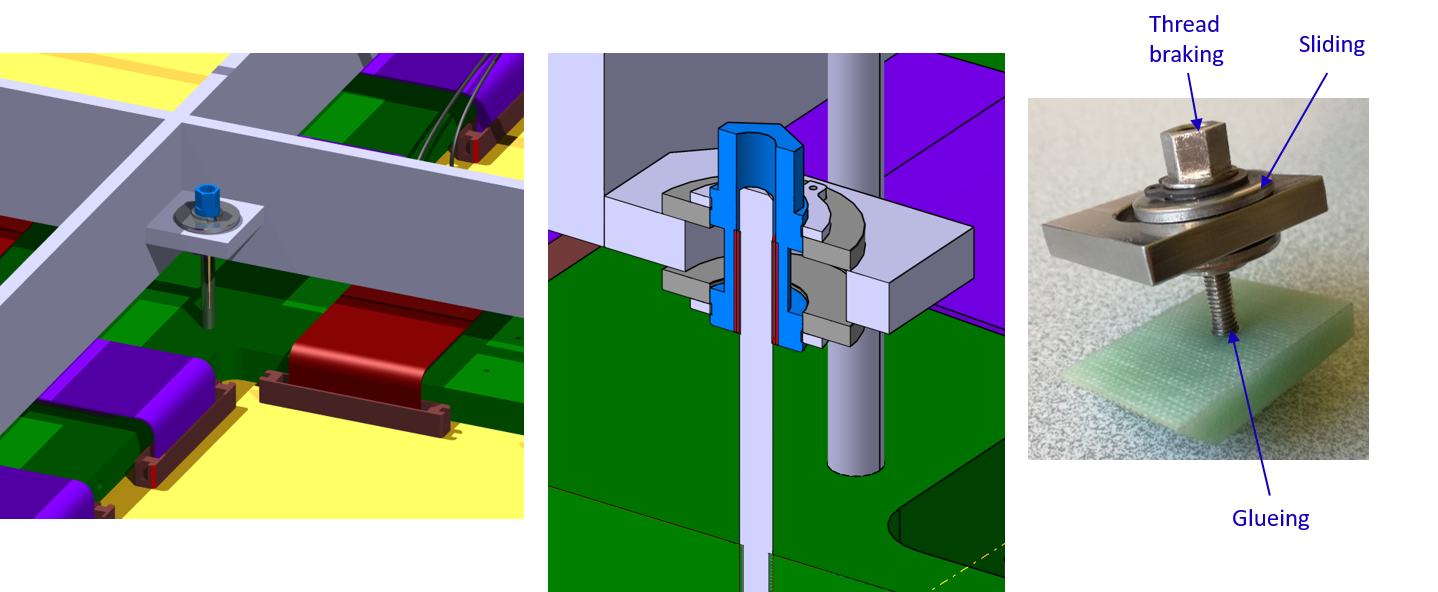
\includegraphics[width=0.8\textwidth]{decoupling.png}
\end{dunefigure}

The full weight of a CRP including the mass of LEMs and anodes is about 330 kg.

%%%%%%%%%%%%%%%%%%%%%%%%%%%%%%%%%%%
\subsection{Extraction grid}
\label{sec:fddp-crp-grid}
The extraction grid consists of 100 μm diameter stainless steel wires tensioned in both x and y directions over the entire 3-m length/width of the CRP with 3.125 mm pitch. They are soldered into groups of 64 on independent wire-tensioning pads oriented perpendicularly to the side of the CRP frame. Each wire-tensioning pad consists of a printed circuit board (PCB)  that is fixed very precisely to a mechanical supporting beams screwed to the G10 frame of the CRP as shown in Figure~\ref{fig:grid-parts}. 
\begin{dunefigure}[optional caption for LoF]{fig:grid-parts}
{Extraction grid components on the CRP structure. On the left the PCB plates and their supporting bars. On the right the system to guarantee the proper wire tensioning with the pushing screws and calibrated wedges to keep the right distance.}
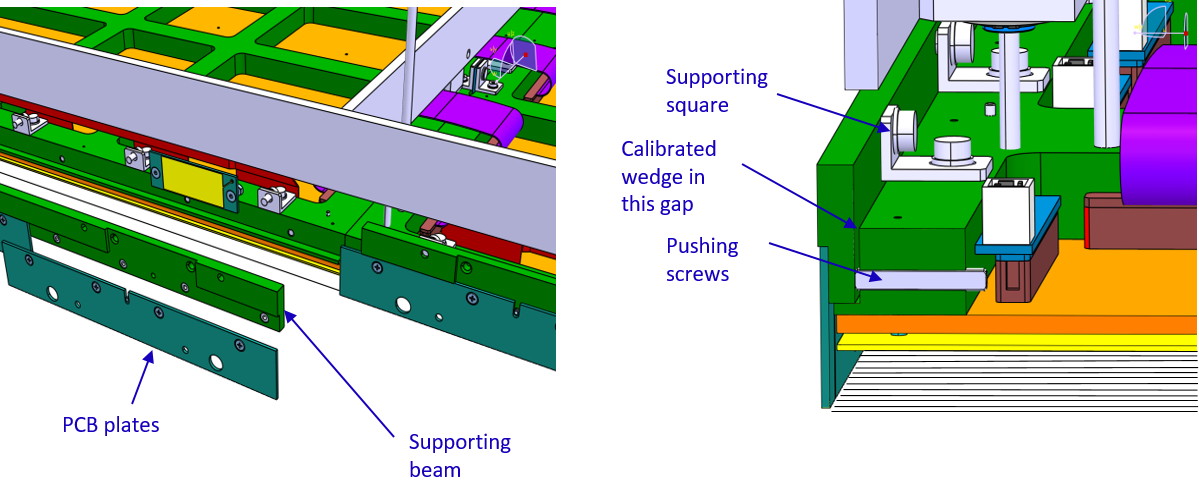
\includegraphics[width=0.8\textwidth]{grid-parts.png}
\end{dunefigure}

The PCB has 64 soldering pads with 200- μm grooves for precise positioning of the wires. During the wire-soldering process each wire is tensioned and positioned in a groove. The PCB is then mounted on the G10 supporting bars and the tension of the group of 64 wires can be precisely adjusted by pushing the supporting bars against the CRP’s G10 frame with screws. The tensioning is performed by tightening «pushing screws», adding a calibrated wedge, and locking the supporting square.
The wires, 3 m long in both x and y directions, have their sags minimized to 0.1 mm thanks to x and y oriented supporting comb-teeth blades  inserted between G10 subframes of 1 m$^2$ size. The array of blades penetrates the liquid surface and has the additional benefit of maintaining the liquid level still.

The grid HV-connection is made through a varnished copper track into two of the 60 PCB plates used for one CRP with a special isolated connection performed inside the CRP structure.


%%%%%%%%%%%%%%%%%%%%%%%%%%%%%%%%%%%
\subsection{Large Electron Multiplier (LEM)}
\label{sec:fddp-crp-lem}
Each LEM consists of a 1\,mm thick, 50$\times$50\,cm$^2$ copper-clad standard PCB epoxy plate. Holes of 500\,$\mu$m diameter, through which electrons undergo amplification, are mechanically drilled in a hexagonal pattern with a pitch of 800\,$\mu$m, yielding about 180 holes per cm$^2$. In addition, each hole has a 40\,$\mu$m dielectric rim, obtained by chemical process, to prevent electrical discharges from occurring near the holes. The holes provide confinement for the UV photons produced during the avalanche process and thus act as a mechanical quencher to prevent photon feedback. This property makes the LEM suitable for operation in ultra-pure argon vapor without the addition of a quenching gas. The final gold plated copper thickness of each LEM electrode is about 60\,$\mu$m. Twenty peripheral and nine central 2.2\,mm diameter holes are used for assembling the LEM module together with its anode on the G10 frame. Figure \ref{fig:LEM_CFR-35} shows a picture of a LEM module used for protoDUNE-DP. To prevent high voltage discharges near or across the edges, the LEM module has a 10\,mm border free from metallization and another 5\,mm copper guard ring. Similar copper guard rings are located around the 2.2\,mm diameter holes and the high voltage connectors. The latter are made with 1.2\,mm diameter male pins (DEUTSCH 6860-201-22278) that are soldered on specifically designed pads imprinted on the LEM electrodes. The pins are insulated with circular tubes made in MACOR and a 10\,mm circular clearance around each pin. 

The total active area of a LEM module used for protoDUNE-DP represents about 86\% of the 50$\times$50\,cm$^2$ area. The choice of the LEM design for protoDUNE-DP was made in order to achieve stable operation conditions up to 3.5\,kV in DLAr mode, corresponding to amplification gains larger than 30 (100) after (before) charging-up of the LEM dielectric material. For the DUNE  10\,kT far detector, a further optimization of the current LEM design will  be performed in order  to find the best compromise between the detector active area and the operation stability.

\begin{figure}[h!]
  \centering
  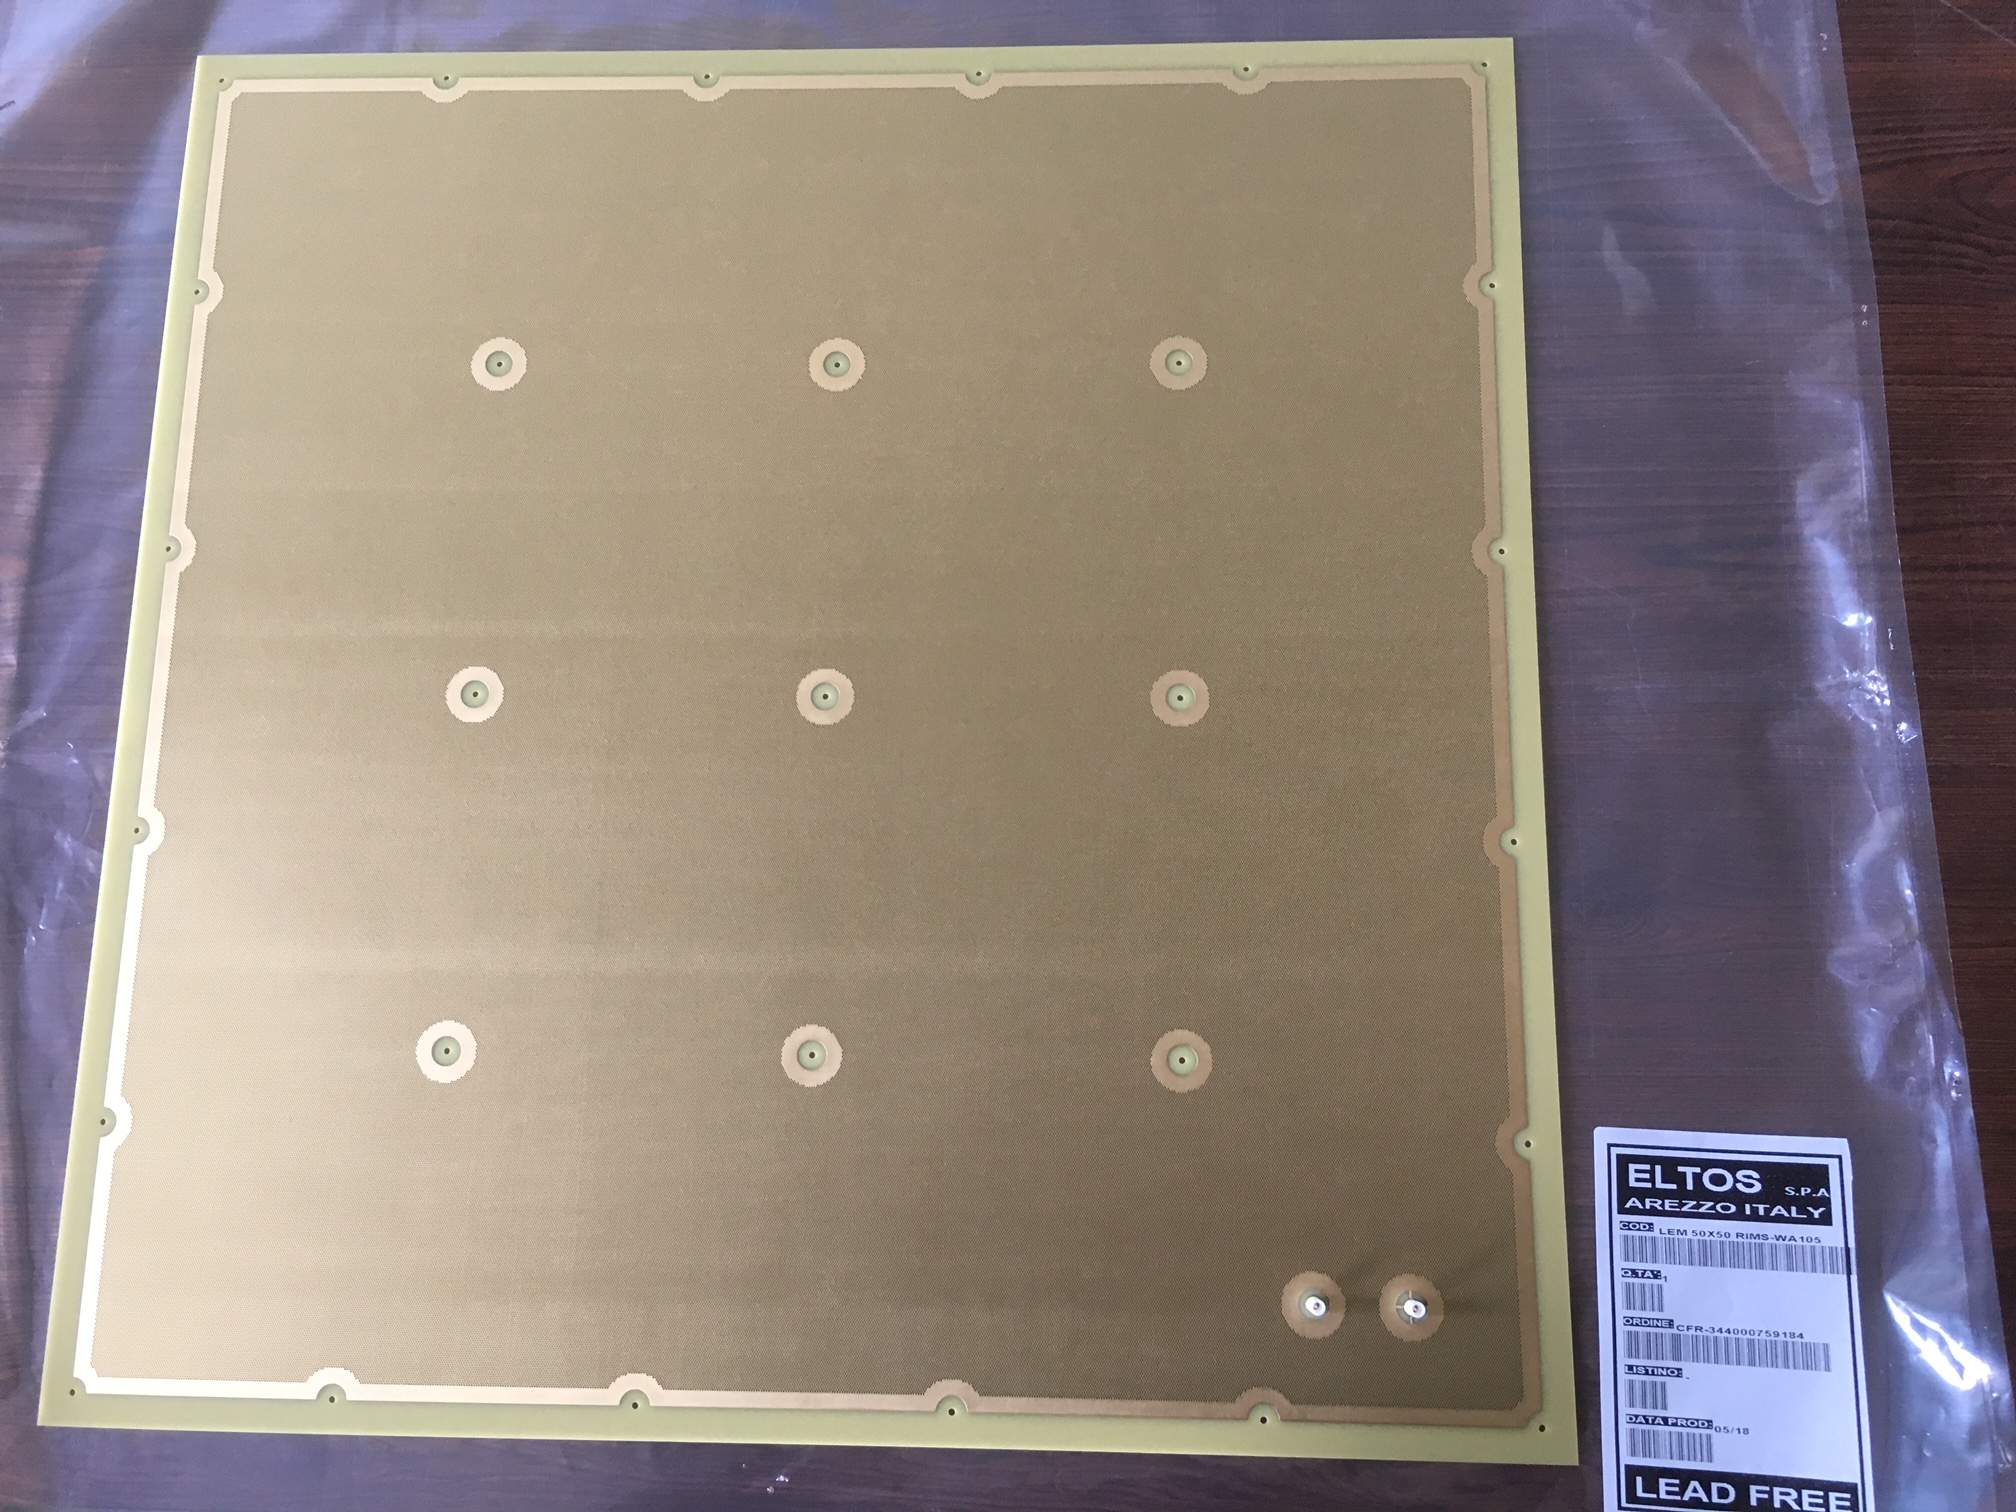
\includegraphics[width=.8\textwidth]{LEM_CFR-35.jpg}
  \caption{Picture of a LEM module used for protoDUNE-DP.}
  \label{fig:LEM_CFR-35} 
\end{figure}

%%%%%%%%%%%%%%%%%%%%%%%%%%%%%%%%%%%
\subsection{Anode}
\label{sec:fddp-crp-anode}
 

The anode is a four-layer PCB having a set of orthogonal strips with a 3.125\,mm pitch that provide the two views of the collected charge. The area of the anode is 50$\times$50\,cm$^2$, identical to the LEM one. Twenty nine holes of 2.2\,mm diameter matching the LEM holes are used for the LEM and anode assembly on their G10 frame. The 2\,mm distance between the anode and the LEM is ensured by 29 precisely machined spacers made of PEEK.

The pattern of the readout strips, printed on the bottom PCB layer and used for charge collection, is optimized such that the charge is evenly split between both views (Figure \ref{fig:Anode}. Electrical insulation in the locations where orthogonal tracks would superimpose is achieved by having tracks crossing over and under each other using a system of vias between the top and bottom layers of the PCB. Each strip, made of thin gold plated copper tracks, has a capacitance per unit length to ground of about 
160\,pF/m. The readout strips are routed to the top layer towards 68-pin female connectors (KEL 8925E-068-179-F) soldered on the anode periphery. Each connector reads 32 strips; its 36 remaining pins are connected to the detector ground via a copper strip which runs around the periphery of the top layer of the anode (see also Figure \ref{fig:Anode_CTest}). 

\begin{figure}[h!]
  \centering
  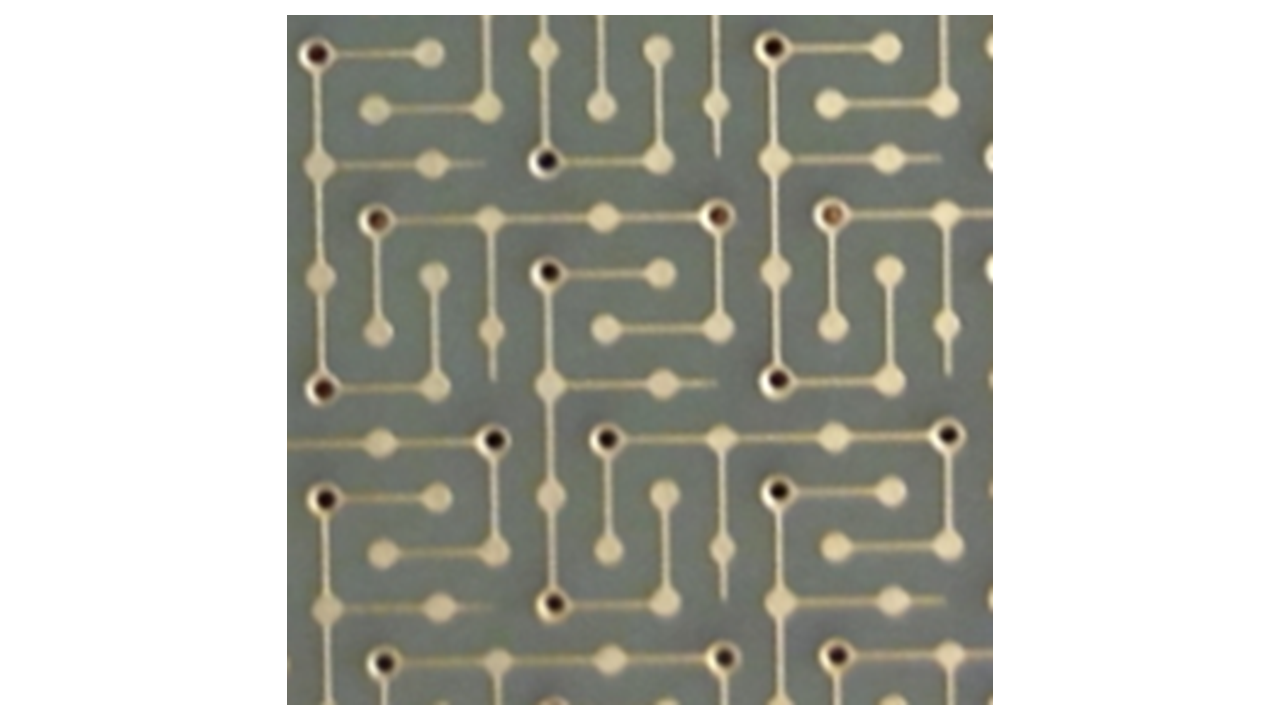
\includegraphics[width=.8\textwidth]{Anode_strips.png}
  \caption{Picture of the anode symmetric two-dimensional strip design.}
  \label{fig:Anode} 
\end{figure}

%%%%%%%%%%%%%%%%%%%%%%%%%%%%%%%%%%
\subsection{Instrumentation}
\label{sec:fddp-crp-instr}

\subsubsection{Distance meters and level meters}
The vertical and lateral positions of the CRP are measured by different means. 
For the vertical position, the use of the suspension system and its motorization on three points will provide an accurate measurement for each CRP of the order of 0.1 mm thanks to the accuracy of the steps motors and encoders. Prior to those measurements the known absolute position of the CRP will be obtained by survey of suspensions and anchor points on the CRP. There will be also the possibility to get relative measurements of the CRP position with respect to the liquid argon level using capacitive level meters put on the sides of the  external CRP of the detection plane. 

The  measurements of the capacitance between the LEM and the extraction grid which depends on the height of liquid above the grid could also give a relative measurement  of the vertical position of the CRP with respect to the liquid surface.

For the lateral measurement of the CRP, capacitive devices called distance meters made of 2 parallel plates will be used for relative alignment of  CRP lateral position. This device gives an accuray of the order of 0.1 mm on the CRP inter distance. 
With these capacitive measurements, no contact is required and four devices per CRP side are embedded in the G10 frame side as can be seen on Figure~\ref{fig:distancemeter}.

\begin{dunefigure}[optional caption for LoF]{fig:distance meter}
{View of the distance meter plates on the sides of a CRP.}
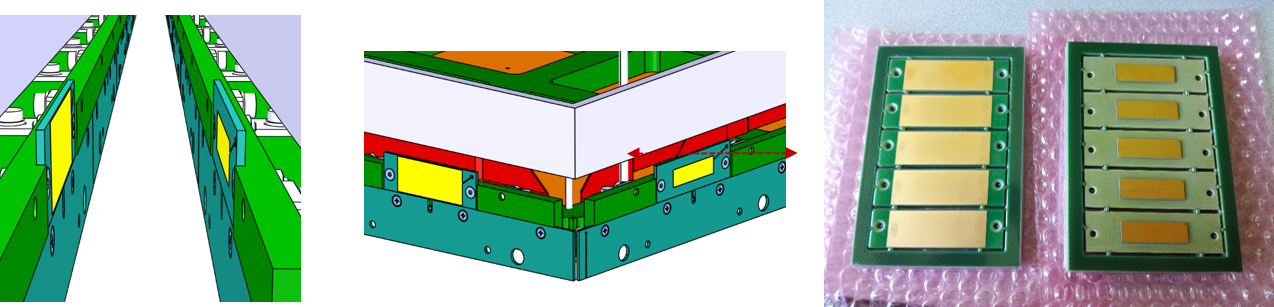
\includegraphics[width=0.85\textwidth]{distancemeter.png}
\end{dunefigure}


\subsubsection{Thermometers}

The temperature in the gas above the anode plane will be monitored at different heights with resistance thermometers (Pt sensors) soldered on  6 PCB boards distributed over the full surface of the CRP.
There will be 6 sensors per PCB. The configuration and the Pt positions are shown in Figure~\ref{fig:ptsensor}.

\begin{dunefigure}[optional caption for LoF]{fig:ptsensor}
{View of the thermometer board and the positions of the Pt sensors along the PCB plate.}
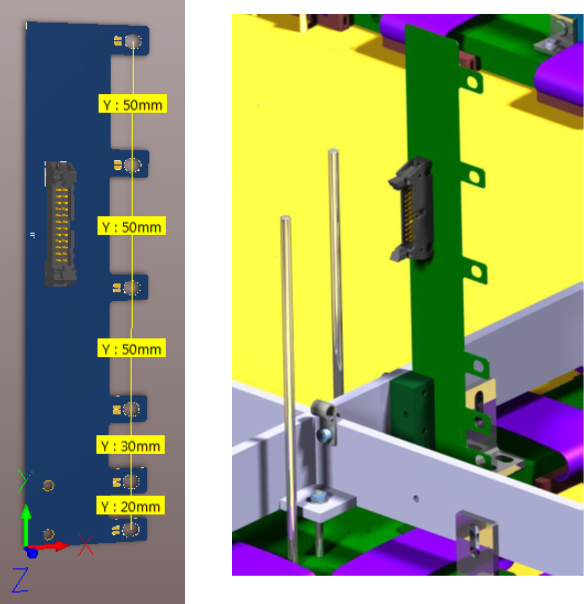
\includegraphics[width=0.35\textwidth]{ptsensor.png}
\end{dunefigure}
%%%%%%%%%%%%%%%%%%%%%%%%%%%%%%%%%%%
\subsection{Suspension system and drive}
\label{sec:fddp-crp-suspension}
Three suspension feedthroughs (SPFT) are arranged as an equilateral triangle whose barycenter coincides with that of the CRP; they suspend the CRP at the required position and precisely adjust the CRP level with respect to the liquid argon surface.

Figure~\ref{fig:spft} shows the design of the suspension feedthrough including the bellow and the motors. There are 3 of them per CRP.

\begin{dunefigure}[optional caption for LoF]{fig:spft}
{Suspension feedthrough and various assembly details.}
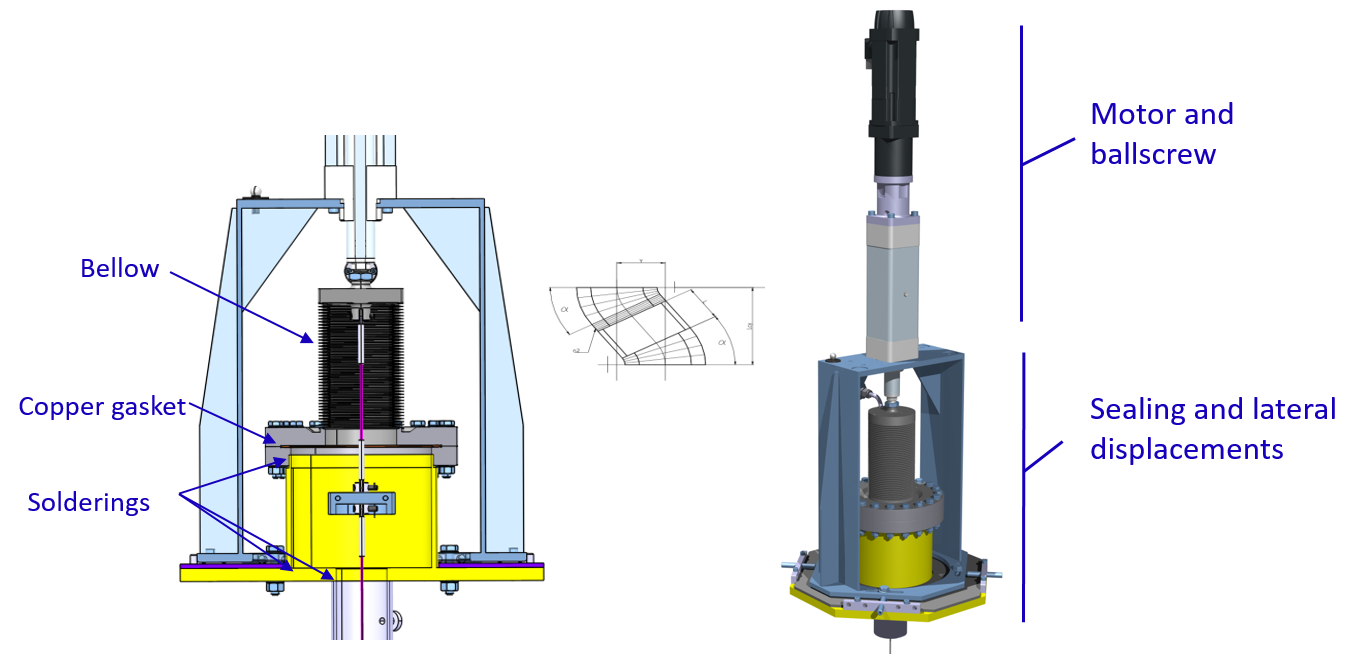
\includegraphics[width=0.7\textwidth]{spft.png}
\end{dunefigure}

At the level of the flanges on the crysotat roof the adjusting table on which the SPFT is screwed allows a lateral stroke of 26mm. Any tranversal movement is absorbed by lateral deformation of the bellow.
The vertical stroke available with the bellow size is $\pm$20mm.
The system incorporates a  Mechanical stop and a simple obstruction of the chimney for maintenance purpose or bellow replacement.
At the top pf the SPFT there is a special slot to positin a  Laser Tracker target
such that the SPFT position can be precisely surveyed during installation.

The suspension cables anchoring system on the CRP is shown in Figure~\ref{fig:anchor}. 
In case of variation of the cryostat pipes verticality, this system allows to change anchoring point on module, in warm conditions. In cold condition, the transversal movement is done with the SPFT position adjustment.
\begin{dunefigure}[optional caption for LoF]{fig:anchor}
{Anchoring system of the suspension cable on the CRP frame.}
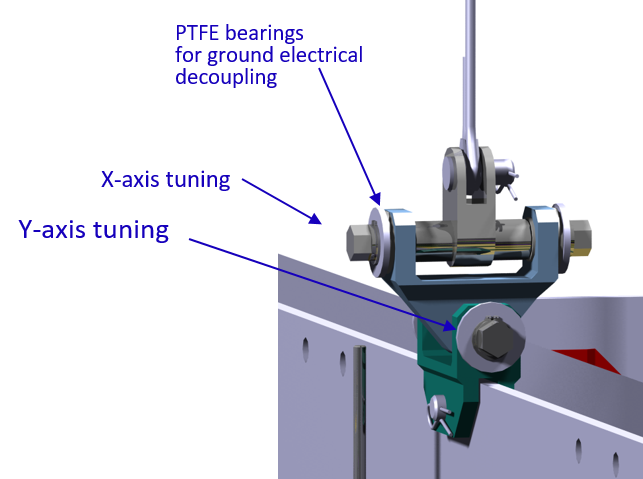
\includegraphics[width=0.6\textwidth]{anchor.png}
\end{dunefigure}

%%%%%%%%%%%%%%%%%%%%%%%%%%%%%%%%%%%
%\subsection{Quality Assurance}
%\label{sec:fddp-crp-qa}

%%%%%%%%%%%%%%%%%%%%%%%%%%%%%%%%%%%%%%%%%%%%%%%%%%%%%%%%%%%%%%%%%%%%
\section{Production and Assembly}
\label{sec:fddp-crp-prod-assy}

%%%%%%%%%%%%%%%%%%%%%%%%%%%%%%%%%%
\subsection{G10 and Invar frame production}
\label{sec:fddp-crp-frame}
G10 and Invar frames are produced by industry
Indicate the number of pieces
Indicate QA acceptance tests (performed by the CRP production centers)

%%%%%%%%%%%%%%%%%%%%%%%%%%%%%%%%%%
\subsection{LEM and anode production}
\label{sec:fddp-crp-LASprod}
The construction of a 10\,kT far detector based on the Dual Phase LAr technology involves the production of 2880 charge readout modules made of a LEM and its anode. For such a large production, it is desirable to use more than one manufacturer in order to mitigate risks and costs. ELTOS in Italy is the company which is making the LEM modules and the anodes for protoDUNE-DP and as such, has worked out successfully the QA/QC process based on requirements and specifications agreed with the WA105 Collaboration. So far, the fraction of rejected LEM modules produced by ELTOS, after the final phase of tests, has proved to be rather small, corresponding to less than one LEM per CRP. The rejection factor for the anodes is, however, larger and corresponds to about 10\%, owing to the very thin and fragile conducting strips forming the anode plane and also to the vicinity of the outer strips with the PCB edges. Small modifications to the anode design will be necessary for DUNE in order to increase the robustness of the manufacturing process. It is believed that such modifications can be envisaged without affecting significantly the performance of the anode.   

A second manufacturer, ELVIA in France, is also known to have the capability for large-scale LEM and anode production with the requested specifications. Recently, several LEM prototypes have indeed been built for CEA/Irfu by ELVIA and extensive tests have shown that the same LEM performance as with ELTOS could be achieved. One key issue for a very large production, like the one necessary for DUNE, is to establish a thorough QA/QC process that can be applied throughout the whole LEM production. The definition of the LEM manufacturing requirements and specifications is naturally an important part of the tendering process. As far as the anodes are concerned, several prototypes have already been manufactured by ELVIA with satisfactory results. Despite the large size (50$\times$50\,cm$^2$) of the anode, its fabrication follows a rather standard process mastered by several PCB manufacturers in Europe and around the world.     

%%%%%%%%%%%%%%%%%%%%%%%%%%%%%%%%%%
\subsubsection{LEM production and QA/QC}
\label{sec:fddp-crp-LEMprod}

In the following scheme, an effective production time of 40 weeks per year and a total duration of two years is assumed. This corresponds to an average LEM production rate of 1 CRP or 36 LEM modules per effective week. The main limitation to the manufacturing speed comes from the LEM drilling process. While it is likely that ELTOS and ELVIA will have the capability each to produce 18 LEM modules per week by assigning dedicated drilling machines, it would still be highly advisable to identify, well before the start of the LEM production phase, additional manufacturers capable of large-scale productions. 

Based on the experience gained with protoDUNE-DP, the QA/QC requirements during the LEM manufacturing process include the selection of the base material for the LEM PCB, thickness measurements of the dielectric material and copper layers before and after the process, a control of the size of the LEM holes, rims and outer dimensions, as 
well as a measurement of the electrical insulation across the two faces of the PCB.  
Table \ref{tab:LEM_Tolerance} gives, as an example, the requested tolerance values on the various parameters of the LEM detectors for protoDUNE-DP. In addition, pre-series productions of several LEM modules from each manufacturing site will be necessary in order to validate the complete fabrication process prior to the start of the full production.

\begin{table}[h!]
\begin{center}
\begin{tabular}{p{.4\textwidth}p{.30\textwidth}}
\hline
\hline
%  & \\ 
 Parameter & Value and tolerance\\
%  & \\ 
\hline
%& \\ 
Dielectric thickness & 1.00$^{+0.00}_{-0.05}$\,mm \\
%  & \\ 
Average total thickness & 1.20$^{+0.00}_{-0.06}$\,mm \\
%  & \\ 
Dimensions & 499.5$^{+0.00}_{-0.30}$\,mm$\times$499.5$^{+0.00}_{-0.30}$\,mm \\
%  & \\ 
Final PCB thickness & 1.10$^{+0.02}_{-0.05}$\,mm \\
%  & \\ 
Active hole diameter & 0.50$^{+0.00}_{-0.01}$\,mm \\
%  & \\ 
Rim size & 40$\pm$4\,$\mu$m \\
%  & \\   
Electrical insulation & > 1\,G$\Omega$ \\
%  & \\   
\hline
\hline
\end{tabular}
\caption{Tolerance values on various LEM parameters }
\label{tab:LEM_Tolerance}
\end{center} 
\end{table} 

Once manufactured, the LEM modules are shipped to one or several Collaboration sites for their final characterization and validation. Several infrastructures are necessary in order to achieve these tasks. Such infrastructures include, for example, a survey bench, clean rooms and storage rooms, cleaning stations and high-voltage test setups. Here is a list of tasks to be performed, in sequential order:
\begin{itemize}
\item {\bf Visual inspection and survey.} Upon reception of the LEM modules from the manufacturing sites, the first operations to be carried out are the visual inspection to examine the quality of the LEM surfaces, and then, the detector survey. The parameters which determine the LEM amplification gain are the thickness of the PCB and the geometry of the holes. It is therefore important to assess the uniformity of these parameters over the entire area of a LEM module. For protoDUNE-DP, this is performed on a sampling basis with the use of a confocal laser scanning microscope (CLSM). Several hundreds of measurements are done in each of 25 predefined locations, distributed uniformly over the LEM surface. With such an optical system, the total LEM and copper layer thicknesses as well as the rim size can be measured with a precision of a few microns. For a very large production as for a 10\,kT detector, the development of a fully automatized survey system is mandatory. 
\item {\bf High voltage connection.} The next step consists in the soldering of the HV connection pins on the two LEM copper surfaces as well as the gluing of insulators made of MACOR around the connectors.
\item {\bf Cleaning and polymerization.} The cleaning operation is an important phase of the LEM preparation. Following a procedure defined by CERN/EP-DT-EF-MP and CEA/Irfu, this is done using an ultrasonic bath at 65$\deg$C with a micro-finishing solution (NGL 17.40 Sp ALU III) for the cleaning of the gold plated copper surfaces of the LEM. It is followed by a rinsing phase with water and then with deionized water sprayed under pressure ($<$\,30\,bar). The LEM is then dried in an oven 
at 60$\deg$C for several hours and then baked for 3 hours up to 160$\deg$C, at a temperature near the glass transition point of the dielectric material. From the cleaning operation on, each LEM is handled via an aluminum frame on which it is mounted in order to avoid any contact with the PCB surfaces. Once cleaned, all LEM modules need in addition to be handled and operated in a clean environment with the use, for example, of a laminar flux.  
\item {\bf High voltage tests.} The final validation of a LEM is obtained after a successful and stable operation in pure argon at room temperature and an absolute pressure of about 3.2-3.3\,bar. For this purpose, a high pressure vessel is used. The argon pressure value is precisely adjusted as a function of the argon temperature inside the vessel in order to reach the same gas density as the one existing in dual phase LAr mode. In such a way, the LEM modules are tested at the same Townsend avalanche operation point as in cold. Figure ~\ref{fig:HP} shows the 360\,L high pressure vessel used at CEA/Irfu for the characterization of the protoDUNE-DP LEM modules. Up to nine LEM modules can be stacked inside this chamber for the HV tests. The HP vessel is also instrumented with front-end electronics and a DAQ system for gain measurements in pure argon. In this configuration, a single LEM is installed with its 2D charge collecting anode inside 
a 50$\times$50$\times$5\,cm$^3$ TPC together with a collimated $^{241}$Am open alpha source mounted on 
the cathode. Figure~\ref{fig:HP_ED} shows an event display of a 5.5\,MeV alpha track observed in pure argon gas at an 
absolute pressure of 1\,bar.
During the LEM validation high-voltage tests, a two-step procedure is followed. After pumping for 
about 60 hours down to a residual pressure of 10$^{-4}$\,mbar, the chamber is filled with dry synthetic air and 
high-voltage up to 4.5\,kV is applied across the LEM in order to 
burn possible residual dust. Then, the vessel is pumped again and pure argon (graded 5.7)
is introduced at an absolute pressure of about 3.2 to 3.3\,bar. Each LEM module is tested 
and validated if it can reach the value of 3.5\,kV across the two faces, consistent with amplification gains higher than 100 before charging up, with no occurrence of discharges. The amount of time needed to perform the HV tests is 
typically one week for an entire batch of 9 LEM modules. This last figure can probably be increased to 12 with a slightly larger volume vessel. 

\end{itemize}
While the tasks related to the LEM visual inspection, survey and the implementation of the HV connections can be done at 
one single Collaboration site, the subsequent operations could be dispatched among several sites. In that case, it is  important that each Collaboration site involved in the final validation steps has the necessary infrastructure for 
both, the cleaning phase and the high voltage tests, as iterations are sometimes necessary in order to fully validate the 
LEM modules. With the assumption of 36 LEM modules produced per effective week, a reasonable number of setups needed for the HV tests, together with their associated instrumentation and infrastructure, could amount to 3 or 4. Finally, based on the experience gained in protoDUNE-DP, the processing time needed for the preparation, characterization and tests of a batch of 9 to 12 LEM modules can be estimated to about 3 weeks.  

\begin{figure}[h!]
  \centering
  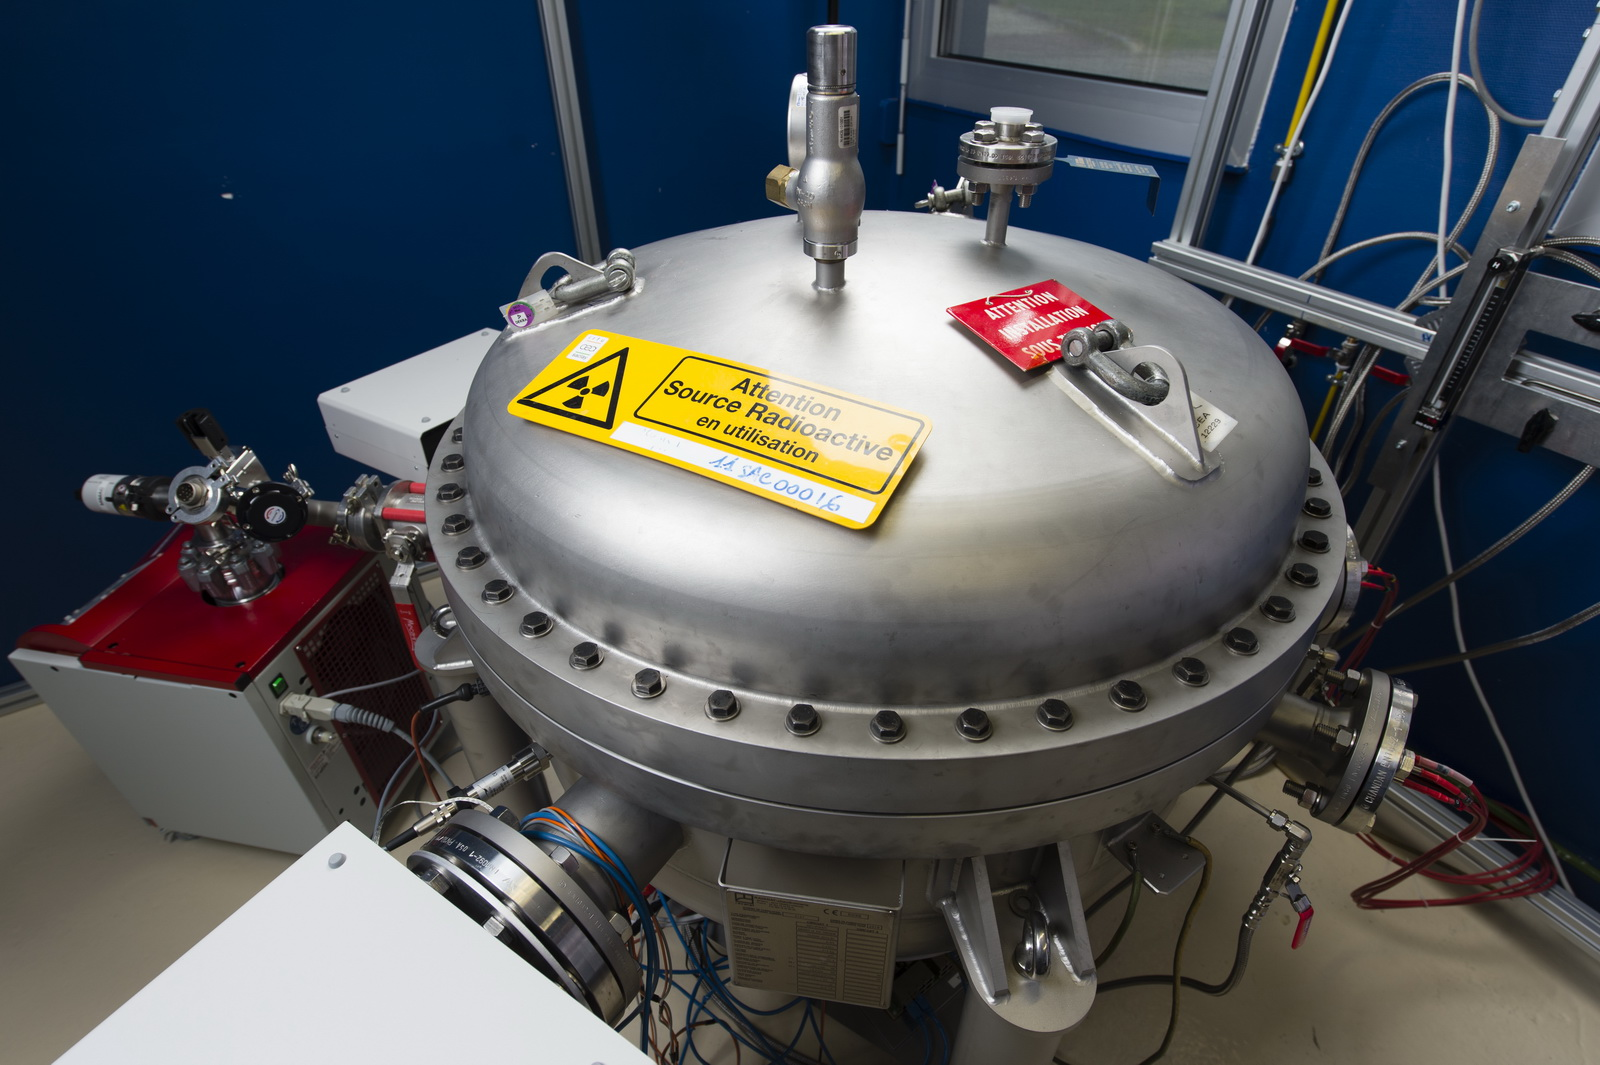
\includegraphics[width=.8\textwidth]{HP.jpg}
  \caption{High-pressure vessel for the characterization of the protoDUNE-DP LEM modules.}
  \label{fig:HP} 
\end{figure}

\begin{figure}[h!]
  \centering
 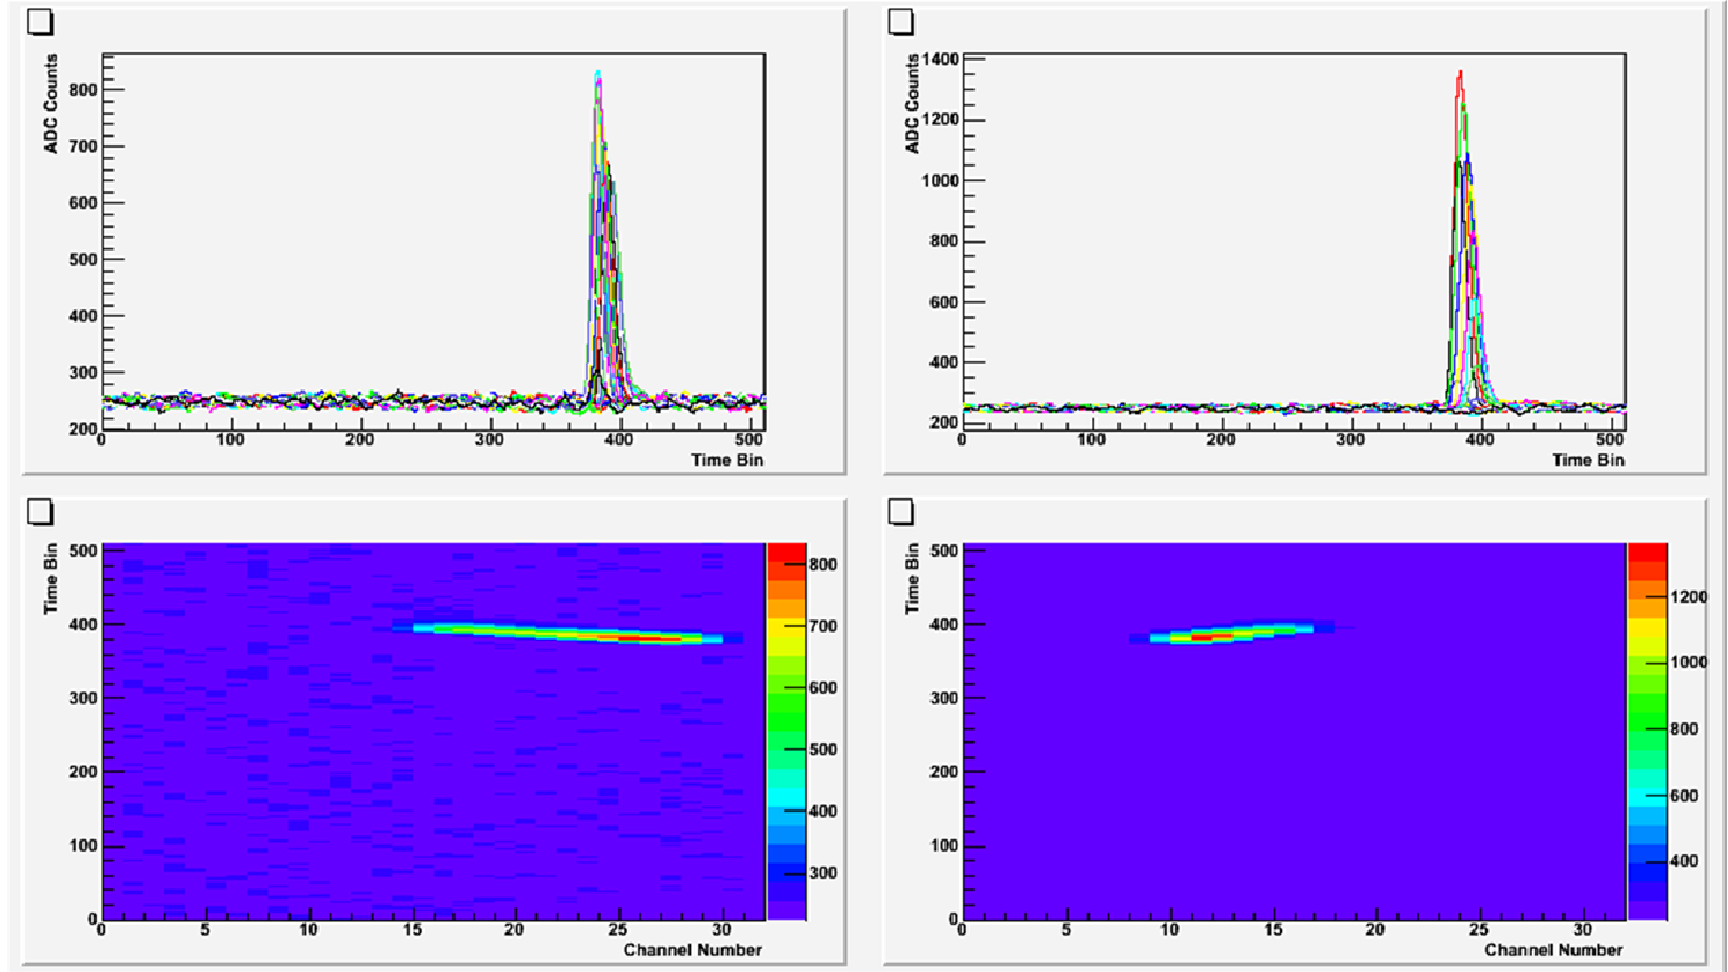
\includegraphics[width=.8\textwidth]{HP_ED.png}
  \caption{Event display of a 5.5\,MeV alpha track in argon gas at 1\,bar.  Left: X-View. Right: Y-View. Top: Pulse-height distributions of hits in ADC counts. Bottom: Hit time [300\,ns bins] -vs- strip number.}
     \label{fig:HP_ED} 
\end{figure}

%%%%%%%%%%%%%%%%%%%%%%%%%%%%%%%%%%
\subsubsection{Anode production and QA/QC}
\label{sec:fddp-crp-ANODEprod}
It is realistically assumed that the lead time in the manufacturing of the anodes will be compatible with the production time
of the LEM modules. Table \ref{tab:ANODE_Tolerance} gives the anode specifications for the dimensions of the PCB. In addition, visual inspection and continuity tests are requested at the manufacturing site after the soldering of the signal connectors. Upon reception at the Collaboration site(s) where the CRP assembly will take place, continuity and short circuit tests of the anode strips are performed (see Figure \ref{fig:Anode_CTest}). This task is rather quick and should not take more than one day per CRP.  

\begin{table}[h!]
\begin{center}
\begin{tabular}{p{.4\textwidth}p{.30\textwidth}}
\hline
\hline
%  & \\ 
 Parameter & Value and tolerance\\
%  & \\ 
\hline
Dimensions & 499.5$^{+0.2}_{-0.0}$\,mm$\times$499.5$^{+0.2}_{-0.0}$\,mm \\
%  & \\ 
PCB thickness & 3.5$\pm$0.05\,mm \\
%  & \\ 
PCB sagitta & < 1\,mm \\
%  & \\   
\hline
\hline
\end{tabular}
\caption{Specifications for the anode dimensions}
\label{tab:ANODE_Tolerance}
\end{center} 
\end{table} 

\begin{figure}[h!]
  \centering
  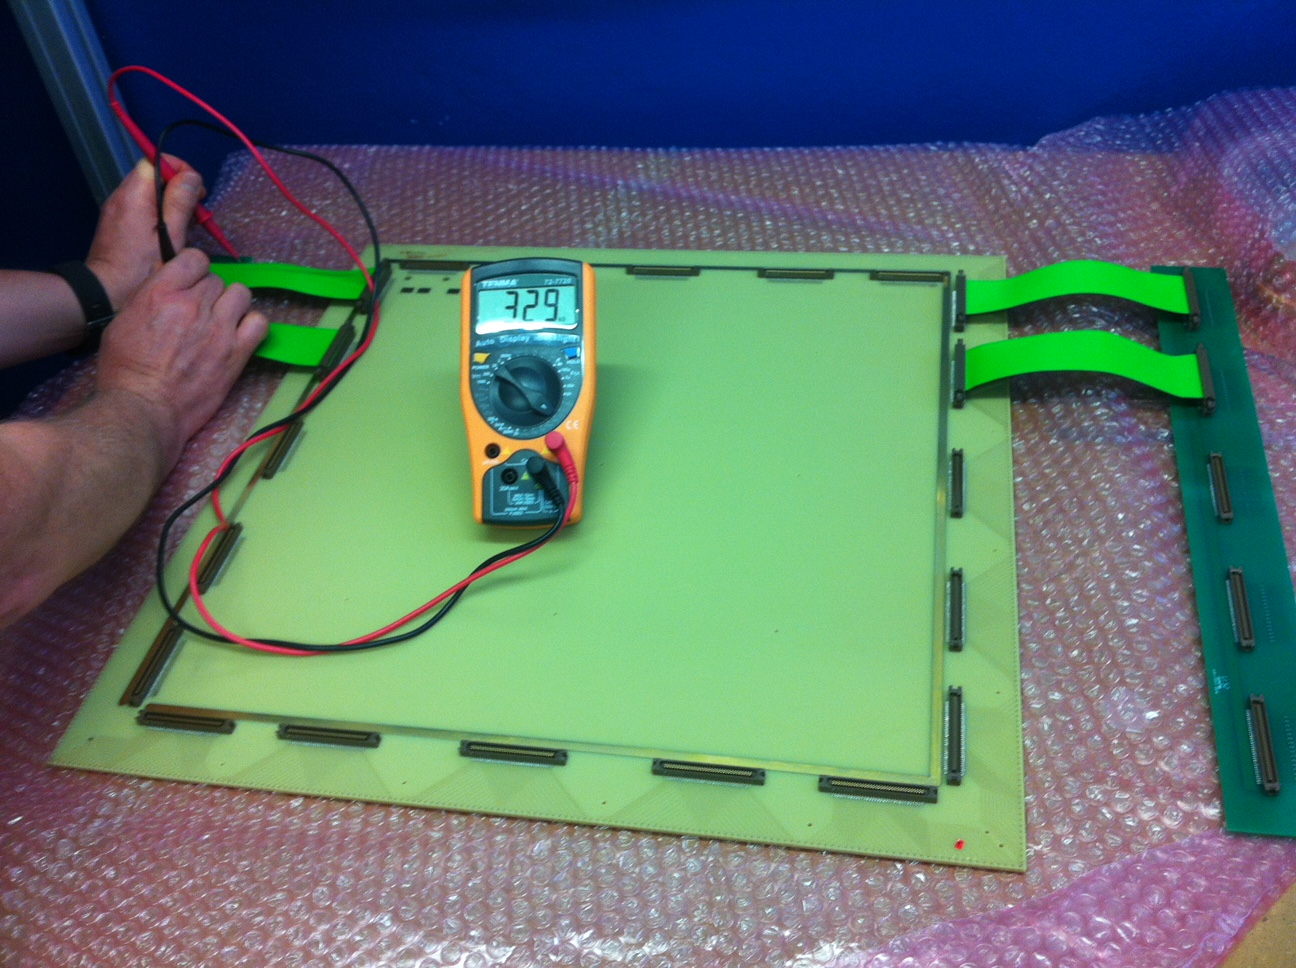
\includegraphics[width=.8\textwidth]{Anode_CTest.jpg}
  \caption{Test of anode strip continuity.}
  \label{fig:Anode_CTest} 
\end{figure}



%%%%%%%%%%%%%%%%%%%%%%%%%%%%%%%%%%
\subsection{Tooling}
\label{sec:fddp-crp-tooling}

\fixme{add description}
Clean room
Assembly tables 
Wiring tools
Storage and transportation boxes


%%%%%%%%%%%%%%%%%%%%%%%%%%%%%%%%%
\subsection{Assembly Procedures}
\label{sec:fddp-crp-assy}

The CRP assembly production activity will span over two years prior to the CRP underground installation. The CRPs will be integrated in at least two different production sites and stored locally in temporary storage boxes before being shipped to the ITF delivery facility. The CRP assembly will be pipelined with the LEM and anodes production and testing during these two production years with an initial  shift of 3 months needed to constitute a large enough LEM and anodes buffer to start the CRP assembly activities.

\fixme{Put here the details of the assembly procedures copied from the example of ProtoDUNE-DP in the clean room 185 with also some cad pictures and pictures of the real tooling and elements. The assembly movie can be also put  as external link.}

An example of the assembly procedures performed for the CRP  construction in the clean room in Building 185 at CERN for ProtoDUNE-DP can be seen at: https://youtu.be/jcnJjlU-Cyc


%%%%%%%%%%%%%%%%%%%%%%%%%%%%%%%%%%%%%%%%%%%%%%%%%%%%%%%%%%%%%%%%%%%%
\section{Interfaces}
\label{sec:fddp-crp-intfc}

The main interfaces with the CRP are linked to the different elements which are connected to them. Namely the readout electronics  (DocDB 6751): It 
concerns the cabling of the signal cables on the bottom part of the cold 
flange of the Signal chimneys.  \\
The Joint Cryogenics Instrumentation and slow controls (DocDB 6760):  it  concerns the power supplies for LEM and extraction grid, the cameras, LED ribbons, temperature sensors, distance meters. All these devices go to the CRP instrumentation feedthroughs. \\

Drift HV (DocDB 6754) at the level of design requirements: it includes the system for maintaining the proper distance between the top most field shaping profile to the extraction grid to keep the proper extraction field and to protect the contact between the two systems.\\

%%%%%%%%%%%%%%%%%%%%%%%%%%%%%%%%%%%
\subsection{TPC Electronics}
\label{sec:fddp-crp-intfc-elec}

The interface with the Dual-Phase TPC electronics is at the level of the bottom flanges of the signal chimneys where the flat cables bringing the signals from the anodes are plugged during the CRP installation in the cryostat. The system which allows pulsing the anode strips is installed by the CRP consortium at the moment of the CRP installations. The strips calibration by using this system is then performed jointly by the two consortia

%%%%%%%%%%%%%%%%%%%%%%%%%%%%%%%%%%%
\subsection{Instrumentation and HV Feed-through flanges}
\label{sec:fddp-crp-intfc-FT}
The 36 LEM modules of a CRP are supplied with high voltage by 42 coaxial cables 
connecting the feed-through flange from the top of the cryostat to distribution boxes located on the CRP (Figure \ref{fig:CRP_DB}). Each cable (20\,AWG, 50\,ohm KAPTON insulated coaxial cable from ACCU-GLASS) can sustain 30\,kV in air and has SHV plugs on each end in order to facilitate connections during the CRP installation.

There are 6 cables used for the LEM top electrodes and 36 cables for the bottom ones. Each of the coaxial cables for the LEM top electrodes is connected to a single distribution box. The later contains a PCB which allows to distribute high voltage to 6 individual LEM modules with a 500\,M$\Omega$ resistor in series for each 
LEM (Figure \ref{fig:LEM_DB}). The 36 coaxial cables for the LEM bottom electrodes are connected by groups of 4 to 9 distributions boxes. In this case, each HV cable is directly linked to an individual LEM bottom electrode. In total, 72 output coaxial cables rated for 10\,kV (26\,AWG, 50\,ohm KAPTON insulated coaxial cable from ACCU-GLASS) are used to supply high voltage to both electrodes of all LEM modules of a CRP. The grounding of each coaxial line is ensured from the feed-through flange down to about 5\,cm from the LEM final connection point via the PCB located inside each of the 15 distribution boxes. In this way, contributions from the HV lines to the electronic noise is limited as much as possible. In order to avoid electrical discharges inside the distribution boxes, the latter are filled with ARATHANE epoxy glue. Finally, the connections to the HV contacts of the LEM modules are done via  DEUTSCH 6862-201-22278 female connectors and each of them is covered by a heat-shrink sleeve. 

\begin{figure}[h!]
  \centering
  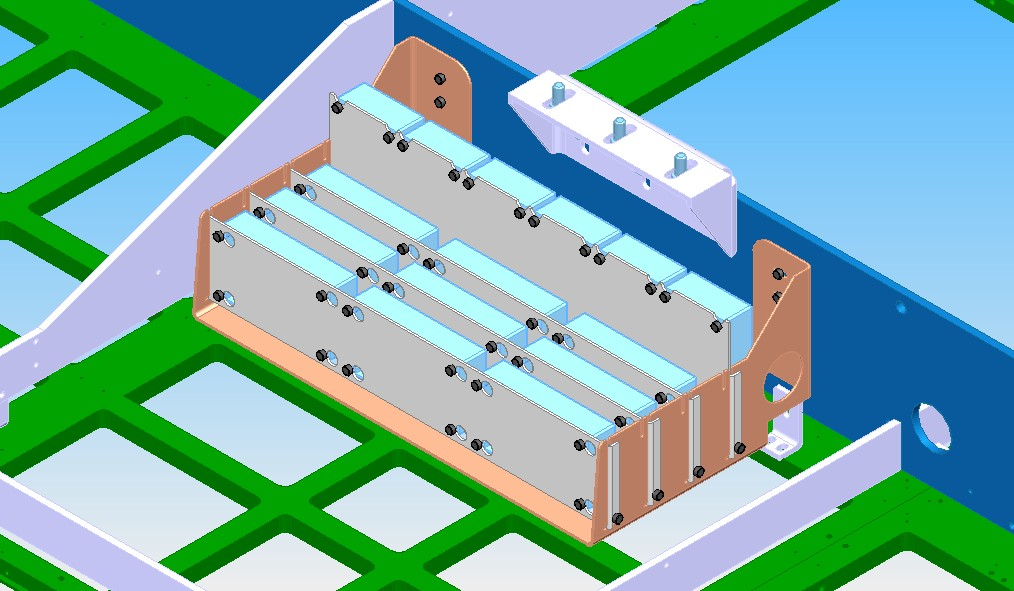
\includegraphics[width=.8\textwidth]{CRP_DB.jpg}
  \caption{LEM high voltage distribution boxes mounted on a CRP.}
  \label{fig:CRP_DB} 
\end{figure}

\begin{figure}[h!]
  \centering
  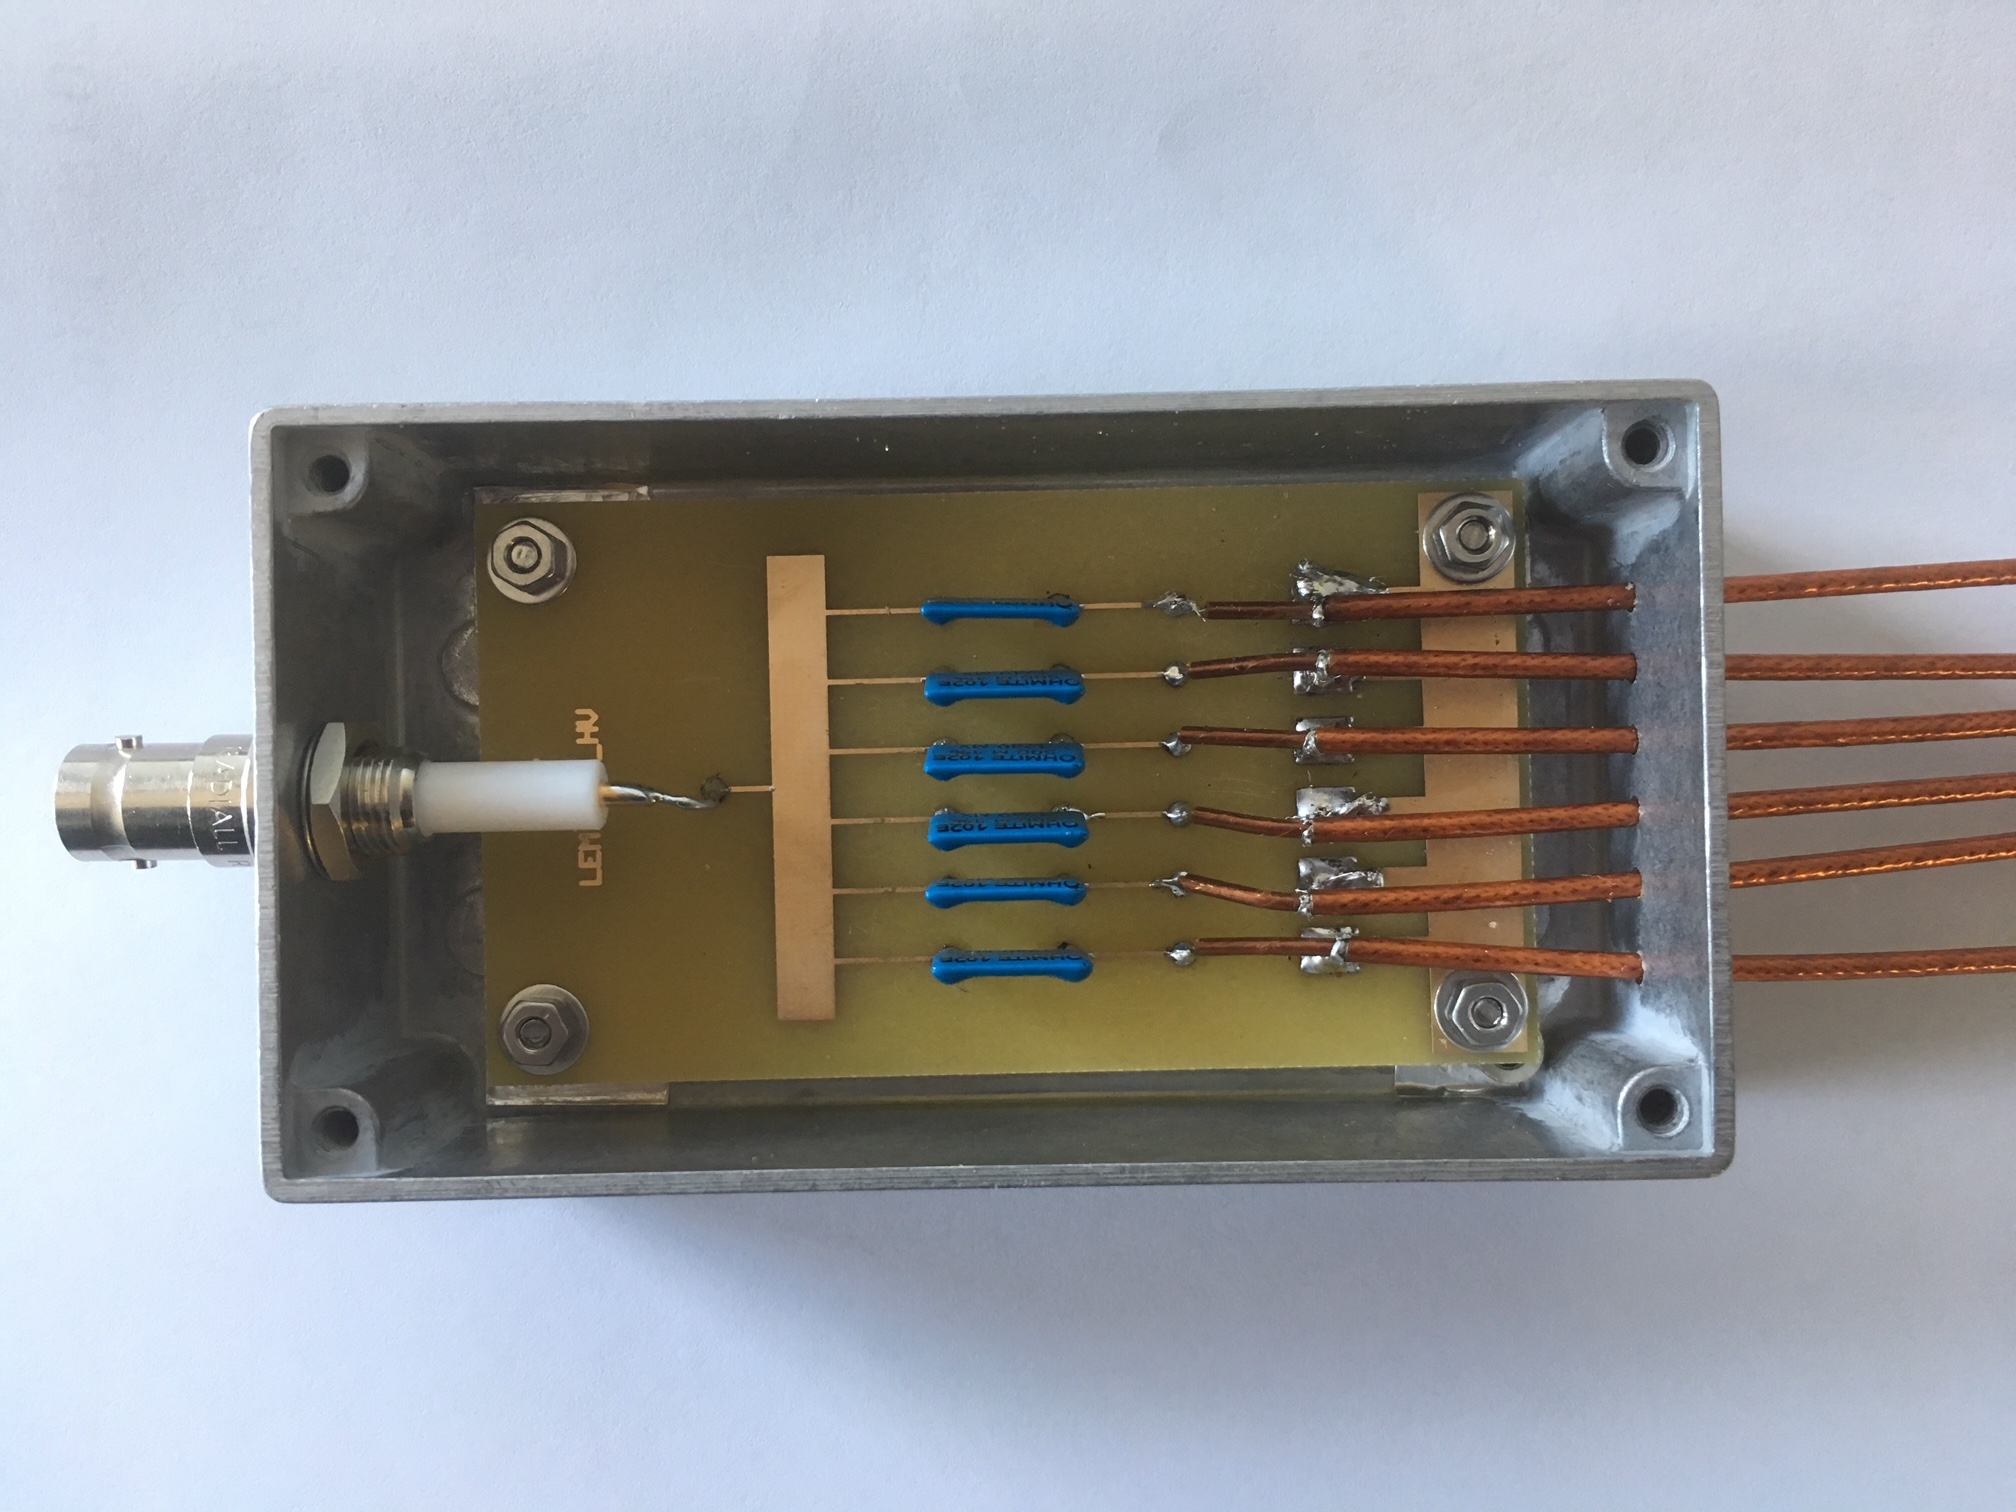
\includegraphics[width=.8\textwidth]{LEM_DB.jpeg}
  \caption{High voltage distribution box for LEM top electrodes before filling with ARATHANE glue.}
  \label{fig:LEM_DB} 
\end{figure}

%%%%%%%%%%%%%%%%%%%%%%%%%%%%%%%%%%%
\subsection{Cryostat/Detector Support Structure}
\label{sec:fddp-crp-intfc-support}

The cryostat includes the dedicated penetrations for the hanging system of each CRP. Each penetration has a diameter of 60mm. The layout of the cryostat penetrations   matches the position of the hanging points on the CRP supporting structure. The penetration flanges and CRP suspension step motors are provided by the CRP consortium.

%%%%%%%%%%%%%%%%%%%%%%%%%%%%%%%%%%%
\subsection{HV/Slow control}
\label{sec:fddp-crp-intfc-HV-slowcontrol}

The interface with the slow control includes:

\begin{itemize}
\item The procurement and control of the power supplies for the HV and grid LEM biasing
\item The control of the CRP temperature probes and level meters
\item The procurement and control of the CRP pulsing system (external to the cryostat)
\item The procurement of the instrumentation and HV feed-through flanges
\item The control of the CRP suspension step motors
\end{itemize}

%%%%%%%%%%%%%%%%%%%%%%%%%%%%%%%%%%%%%%%%%%%%%%%%%%%%%%%%%%%%%%%%%%%%
\section{Installation, Integration and Commissioning}
\label{sec:fddp-crp-install}

The installation of the CRPs in the cryostat will be performed on a time span of 8 months, following the installation of the signal chimneys which will take 3 months. The presence of the signal chimneys is needed in order to be able to connect the CRP signal flat cables. The suspension, instrumentation and HV flanges must also be already installed at the moment of the CRP installation. The installation of these flanges can be performed in parallel to the installation of the signal chimneys. The production of the CRPs will be performed before the installation and the CRPs will be stored in temporary storage boxes at the production centers. During installation the already produced CRPs will be moved to the transportation boxes in order to be shipped to the ITF and then moved underground. Given the installation rate of 8 CRPs/month a set of 30 transportation boxes will ensure a sufficient turnover among the production sites and the installation site.

The installation procedure foresees the operation from 3 teams (2 persons/team) working in parallel inside the cryostat to manage the installation of 3 CRPs at the same time. It is assumed that of the order of 1.3 weeks will be needed for a team to prepare, survey, tune, cable a CRP in the  cryostat and 35 working weeks for the overall installation of the 80 CRPs.

Once the 3 CRPs are ready to be lifted, 3 persons are needed to manipulate the manual winches on the top of the cryostat for a few hours. This activity should occur during the 1.3 weeks period just before the cabling activity for the connection to the flanges.

\fixme{Put here more details of the different steps for the underground installation/ positioning of the box, suspension of the CRP, cabling at height, etc .. and the associated tooling !}

%%%%%%%%%%%%%%%%%%%%%%%%%%%%%%%%%%%%
\subsection{Transport and Handling}
\label{sec:fddp-crp-install-transport}

The transportation boxes are sized for the shafts and underground handling at SURF (provide here the external envelope of the box). They will be protected by a plastic layer which should be removed once the transportation box arrived to the gray room area underground in order that the box in a clean state can be introduced in the cryostat via the TCO. The transportation box is also essential to handle the CRP from the vertical (insertion in the TCO) to the horizontal position in which the CRP should be prior to its hanging to the suspension system. Once the installation is completed the transportation boxes should be wrapped again with a protective layer and shipped back to the production centers. 

%%%%%%%%%%%%%%%%%%%%%%%%%%%%%%%%%%%
\subsection{Calibration}
\label{sec:fddp-crp-install-calib}

The CRP calibration relies on a pulsing system which performs charge injection in the strips via 1 pF capacitors. The pulse distribution system and related cabling and the boards with the charge injection capacitors are integrated  with the CRP at the time of the CRP assembly. At the time of the CRP assembly this system is connected via flat cables to the instrumentation flange. An pulsing distribution system external to the cryostat and  provided by the slow control consortium ensures the driving of the charge injection system.  The information from the pulse calibration is then complemented with the one from the front-end electronics calibration and the one from the analysis of the reconstructed charged tracks in order to extract the overall calibration constants per channel.


%%%%%%%%%%%%%%%%%%%%%%%%%%%%%%%%%%%%%%%%%%%%%%%%%%%%%%%%%%%%%%%%%%%%
\section{Quality Control}
\label{sec:fddp-crp-qc}

Several QA procedures are applied at the level of the LEM and anodes production, as described in more details in the related sections. The components of the HV distribution system are also individually tested. Continuity tests are performed at the time of the CRP assembly. The CRP geometry is also systematically surveyed as well as the tensioning of the grid wires. On a small subsample of the CRPs production it will be also possible to perform cold-box testing by using the infrastructure set up at CERN for ProtoDUNE-DP.


%%%%%%%%%%%%%%%%%%%%%%%%%%%%%%%%%%%%
%\subsection{Protection and Assembly (Local)}
%\label{sec:fddp-crp-qc-local}


%%%%%%%%%%%%%%%%%%%%%%%%%%%%%%%%%%%
%\subsection{Post-factory Installation (Remote)}
%\label{sec:fddp-crp-qc-remote}



%%%%%%%%%%%%%%%%%%%%%%%%%%%%%%%%%%%%%%%%%%%%%%%%%%%%%%%%%%%%%%%%%%%%
\section{Safety}
\label{sec:fddp-crp-safety}

The CRP installation and operation does not present particular safety issues apart working at height during the CRP installation for the connection of the cabling to the signal feed-through chimneys and the instrumentation and HV feedthroughs.

%%%%%%%%%%%%%%%%%%%%%%%%%%%%%%%%%%%
% add subsections and labels if needed \subsection{}
%\label{sec:fddp-crp-safety-}


%%%%%%%%%%%%%%%%%%%%%%%%%%%%%%%%%%
%\subsection{}
%\label{sec:fddp-crp-safety}



%%%%%%%%%%%%%%%%%%%%%%%%%%%%%%%%%%%%%%%%%%%%%%%%%%%%%%%%%%%%%%%%%%%%
%\section{Organization and Management}
%\label{sec:fddp-crp-org}

%%%%%%%%%%%%%%%%%%%%%%%%%%%%%%%%%%%
%\subsection{CRP Consortium Organization}
%\label{sec:fddp-crp-org-consortium}


%%%%%%%%%%%%%%%%%%%%%%%%%%%%%%%%%%
%\subsection{Planning Assumptions}
%\label{sec:fddp-crp-org-assmp}


%%%%%%%%%%%%%%%%%%%%%%%%%%%%%%%%%%%
%\subsection{WBS and Responsibilities}
%\label{sec:fddp-crp-org-wbs}

%%%%%%%%%%%%%%%%%%%%%%%%%%%%%%%%%%
%\subsection{High-level Cost and Schedule}
%\label{sec:fddp-crp-org-cs}














